%%%%%%%%%%%%%%%%%%%%%definitions%%%%%%%%%%%%%%%%%%%%%%%%%%%%%%%%%%%%%%%
%\documentclass[12pt]{article}
%\documentclass[12pt]{scrartcl}
\documentclass{hitec} % contained in texlive-latex-extra
\settextfraction{0.9} % indent text
\usepackage{csquotes}
\usepackage[hidelinks]{hyperref} % doi links are short and usefull?
\hypersetup{%
    colorlinks=true,
    linkcolor=blue,
    urlcolor=magenta
}
\urlstyle{rm}
\usepackage[english]{babel}
\usepackage{mathtools} % loads and extends amsmath
\usepackage{amssymb}
% packages not used
%\usepackage{graphicx}
%\usepackage{amsthm}
%\usepackage{subfig}
\usepackage{bm}
\usepackage{longtable}
\usepackage{booktabs}
\usepackage{ragged2e} % maybe use \RaggedRight for tables and literature?
\usepackage[table]{xcolor} % for alternating colors
%\rowcolors{2}{gray!25}{white} %%% Use this line in front of longtable
\renewcommand\arraystretch{1.3}
\usepackage[most]{tcolorbox}
\usepackage{doi}
\usepackage[sort,square,numbers]{natbib}
\bibliographystyle{abbrvnat}
%%% reset bibliography distances %%%
\let\oldthebibliography\thebibliography
\let\endoldthebibliography\endthebibliography
\renewenvironment{thebibliography}[1]{
  \begin{oldthebibliography}{#1}
    \RaggedRight % remove if justification is desired
    \setlength{\itemsep}{0em}
    \setlength{\parskip}{0em}
}
{
  \end{oldthebibliography}
}
%%% --- %%%

\definecolor{light-gray}{gray}{0.95}
\newcommand{\code}[1]{\colorbox{light-gray}{\texttt{#1}}}
\newcommand{\eps}{\varepsilon}
\renewcommand{\d}{\mathrm{d}}
\renewcommand{\vec}[1]{{\boldsymbol{#1}}}
\newcommand{\dx}{\,\mathrm{d}x}
%\newcommand{\dA}{\,\mathrm{d}(x,y)}
%\newcommand{\dV}{\mathrm{d}^3{x}\,}
\newcommand{\dA}{\,\mathrm{dA}}
\newcommand{\dV}{\mathrm{dV}\,}

\newcommand{\Eins}{\mathbf{1}}

\newcommand{\ExB}{$\bm{E}\times\bm{B} \,$}
\newcommand{\GKI}{\int d^6 \bm{Z} \BSP}
\newcommand{\GKIV}{\int dv_{\|} d \mu d \theta \BSP}
\newcommand{\BSP}{B_{\|}^*}
\newcommand{\Abar}{\langle A_\parallel \rangle}
%Averages
\newcommand{\RA}[1]{\left \langle #1 \right \rangle} %Reynolds (flux-surface) average
\newcommand{\RF}[1]{\widetilde{#1}} %Reynolds fluctuation
\newcommand{\FA}[1]{\left[\left[ #1 \right]\right]} %Favre average
\newcommand{\FF}[1]{\widehat{#1}} %Favre fluctuation
\newcommand{\PA}[1]{\left \langle #1 \right\rangle_\varphi} %Phi average

%Vectors
\newcommand{\ahat}{\bm{\hat{a}}}
\newcommand{\bhat}{\bm{\hat{b}}}
\newcommand{\chat}{\bm{\hat{c}}}
\newcommand{\ehat}{\bm{\hat{e}}}
\newcommand{\bbar}{\overline{\bm{b}}}
\newcommand{\xhat}{\bm{\hat{x}}}
\newcommand{\yhat}{\bm{\hat{y}}}
\newcommand{\zhat}{\bm{\hat{z}}}

\newcommand{\Xbar}{\bar{\vec{X}}}
\newcommand{\phat}{\bm{\hat{\perp}}}
\newcommand{\that}{\bm{\hat{\theta}}}

\newcommand{\eI}{\bm{\hat{e}}_1}
\newcommand{\eII}{\bm{\hat{e}}_2}
\newcommand{\ud}{\mathrm{d}}

%Derivatives etc.
\newcommand{\pfrac}[2]{\frac{\partial#1}{\partial#2}}
\newcommand{\ffrac}[2]{\frac{\delta#1}{\delta#2}}
\newcommand{\fixd}[1]{\Big{\arrowvert}_{#1}}
\newcommand{\curl}[1]{\nabla \times #1}

\newcommand{\np}{\vec{\nabla}_{\perp}}
\newcommand{\npc}{\nabla_{\perp} \cdot }
\newcommand{\nc}{\vec\nabla\cdot}
\newcommand{\cn}{\cdot\vec\nabla}
\newcommand{\vn}{\vec{\nabla}}
\newcommand{\npar}{\nabla_\parallel}

\newcommand{\GAI}{\Gamma_{1}^{\dagger}}
\newcommand{\GAII}{\Gamma_{1}^{\dagger -1}}
\newcommand{\T}{\mathrm{T}}
\newcommand{\Tp}{\mathcal T^+_{\Delta\varphi}}
\newcommand{\Tm}{\mathcal T^-_{\Delta\varphi}}
\newcommand{\Tpm}{\mathcal T^\pm_{\Delta\varphi}}
%%%%%%%%Some useful abbreviations %%%%%%%%%%%%%%%%
\def\feltor{{\textsc{Feltor }}}

\def\fixme#1{\typeout{FIXME in page \thepage :{#1}}%
 \textsc{\color{red}[{#1}]}}


%%%%%%%%%%%%%%%%%%%%%%%%%%%%%DOCUMENT%%%%%%%%%%%%%%%%%%%%%%%%%%%%%%%%%%%%%%%

\begin{document}

\title{DG methods on structured grids}
\author{M.~Wiesenberger}

\section{ Introduction to discontinuous Galerkin methods} \label{sec:discretization}
This writeup is based on Reference~\cite{WiesenbergerPhD}. A useful book to consult
is Reference~\cite{NodalDG}.

In recent years, discontinuous Galerkin (dG) methods have been investigated 
as an excellent alternative to finite difference and finite volume schemes 
in numerical simulations involving both parabolic as well as hyperbolic problems 
(for the advection dominated case see, for example, the review article~\cite{Cockburn2001runge}). 
Such methods combine many advantages of finite element methods (such as the ease of handling 
complicated geometry) with properties more commonly associated with 
finite difference approximations. Examples of the latter includes the absence 
of a global mass matrix. 
The main idea of a dG method is to approximate the solution 
of a differential equation by a polynomial in each grid-cell. 
Higher/lower
order methods can be constructed by simply increasing/decreasing the degree of 
the polynomials used in each cell. 
In classical finite element methods continuity is required across cell boundaries. 
In contrast, dG methods allow discontinuities across cell boundaries, which adds to the flexibility of the method.

For the discretization of second derivatives we discuss the so-called local discontinuous Galerkin (LDG) method~\cite{Cockburn1998}.
The LDG method and its advantages can also be used for the discretization of 
elliptic equations (including Poisson's equation). 
Reference~\cite{Arnold2002} highlights the relation 
of the method to interior penalty and other alternative methods. 
A superconvergence result for the 
LDG approach was proven on Cartesian grids~\cite{Cockburn2002},
where the order of convergence is $1/2$ better than on arbitrary meshes.
Reference~\cite{Yadav2013} later showed a similar result for general, nonlinear elliptic equations.

The downside of the dG methods is their rather complex and unintuitive notation 
in the existing mathematical literature. Often, algorithms
are described in terms of arbitrary sets of polynomials and spatial grids. 
We propose an adapted, simplified, and in our view more practical notation for orthogonal grids and Legendre polynomials, which can be implemented straightforwardly.
We reformulate the LDG method in terms of adjoint matrices and
 naturally develop the symmetry of the resulting discretization.
Doing so, we also propose a new discretization for the general elliptic equation. 
Unfortunately, our discretization has a wider stencil than the existing ones, but 
our numerical experiments indicate superconvergent properties and the resulting
matrix equation is better conditioned than the old one. To the knowledge
of the author these findings are unpublished to date.

\subsection{ The Legendre polynomials} \label{sec:legendre}
First, let us consider the one-dimensional case.
For simplicity and ease of implementation we choose an equidistant grid with $N$ cells $C_n = [x_{n-1/2},x_{n+1/2}]$ of size $h$;
with this choice we are able to construct basis functions of $P(C_n)$, the space of 
polynomials of degree at most $P-1$ on $C_n$, by using orthogonal Legendre polynomials\footnote{ Often, in the literature the order of the polynomials is denoted by $k$.
Pay attention, that we use the number of polynomial coefficients $P$ instead. We have $P=k+1$}.
The Legendre polynomials can be recursively defined on $[-1,1]$ by setting
$p_0(x) = 1$, $p_1(x) = x$ and (see e.g.~\cite{AS})
\begin{align}
    (k+1)p_{k+1}(x) = (2k+1)xp_k(x) - kp_{k-1}(x).
    \label{eq:recursion}
\end{align}
The so constructed Legendre polynomials are orthogonal on $[-1,1]$.
We write
$x^a_j$ and $w_j$, $j=0,\dots,P-1$ denoting the abscissas and weights of
the Gauss--Legendre quadrature on the interval $[-1,1]$. Then we note that for $k,l=0, \dots, P-1$
\begin{align}
    \int_{-1}^1 p_k(x)p_l(x) \dx = \sum_{j=0}^{P-1} w_jp_k (x^a_j)p_l(x^a_j) = \frac{2}{2k+1}\delta_{kl}, 
    \label{}
\end{align}
 since Gauss--Legendre quadrature is exact for polynomials of degree at most $2P-1$.

The discrete completeness relation can then be written as
\begin{align}
    \sum_{k=0}^{P-1} \frac{2k+1}{2}w_j p_k(x^a_i)p_k(x^a_j) = \delta_{ij}.
    \label{eq:completeness}
\end{align}
Given a real function $f:[-1,1]\rightarrow \mathbb{R}$ we define $f_j:=f(x^a_j)$ and
\begin{align} \label{eq:ex2}
    \bar f^k := \frac{2k+1}{2}\sum_{j=0}^{P-1}w_j p_k(x^a_j) f_j
\end{align}
Now let us define the forward transformation matrix by $F^{kj}:=\frac{2k+1}{2}w_jp_k(x^a_j)$ and
the backward transformation matrix by $B_{kj}:= p_j(x^a_k)$.
\begin{tcolorbox}[title=Note]
Reference~\cite{NodalDG} identifies $B$ as the Vandermonde matrix and further denotes $f_i$ as the \textbf{nodal} representation and $\bar f^k$ as the \textbf{modal} representation of $f(x)$.
\end{tcolorbox}

Then, using Eq.~\eqref{eq:ex2}, we get
\begin{subequations}
\begin{align}
    \bar f^k = \sum_{j=0}^{P-1}F^{kj}f_j \\
    f_j = \sum_{k=0}^{P-1} B_{jk}\bar f^k,
\end{align}
\end{subequations}
We call $\bar f^k$ the values of $f$ in $L$-space and $f_j$ the values of $f$ in $X$-space.

Let us now consider an interval $[a,b]$ and an equidistant discretization
by $N$ cells with cell center $x_n$ and grid size $h=\frac{b-a}{N}$; in addition, we set $x_{nj}^a := x_n + \frac{h}{2}x^a_j$.
Given a function $f:[a,b]\rightarrow \mathbb{R}$ we then define
$f_{nj} := f(x^a_{nj})$ and note that
\begin{subequations}
\begin{align}
    \bar{ \vec f} &= (\Eins\otimes F) \vec f \\
    \vec f &= (\Eins\otimes B) \bar{\vec f},
    \label{}
\end{align}
\end{subequations}
where $f_{nj}$ are the elements of $\vec f$,
 $\Eins\in\mathbb{R}^{N\times N}$ is the identity matrix and $F,B\in\mathbb{R}^{P\times P}$. Furthermore, we use
$\otimes$ to denote the Kronecker product which is bilinear and associative. 
The discontinuous Galerkin expansion $f_h$ of a function $f$ in the interval $[a,b]$ can 
then readily be given as
\begin{align}
    f_h(x) = \sum_{n=1}^N \sum_{k=0}^{P-1} \bar f^{nk} p_{nk}(x),
    \label{eq:dgexpansion}
\end{align}
where
\begin{align}
    p_{nk}(x) := \begin{cases}
        p_k\left(  \frac{2}{h}(x-x_n)\right),& \ \text{for } x-x_n\in\left[ -\frac{h}{2}, \frac{h}{2} \right]\\
        0,& \ \text{else}.
    \end{cases}
    \label{}
\end{align}
As an example, we plot Eq.~\eqref{eq:dgexpansion} for $f(x)=\sin(2x)$ in Fig.~\ref{fig:discretization}. 
\begin{figure}[htpb]
    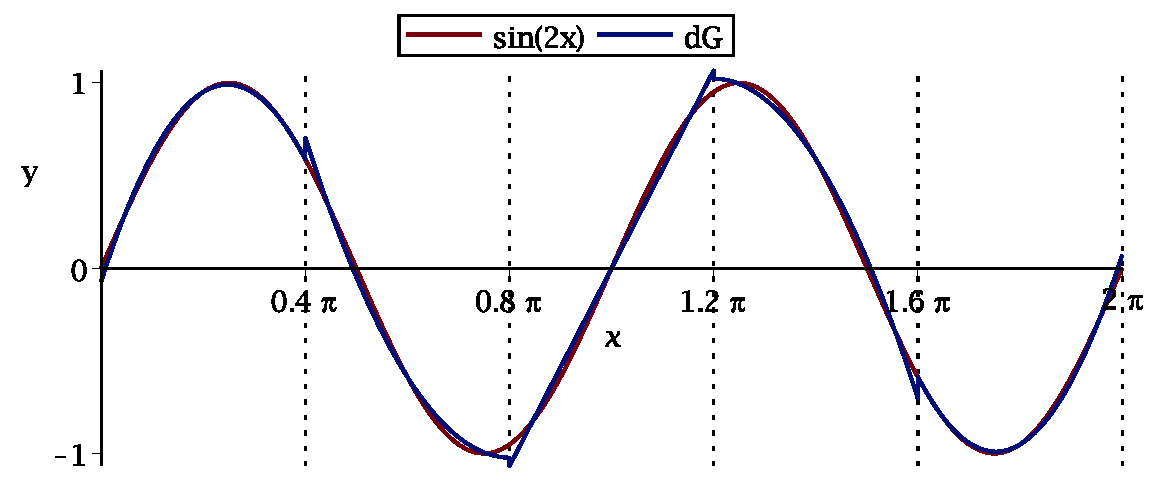
\includegraphics[width= 0.9\textwidth]{discretization.pdf}
    \caption{ 
    Discretization of a sine function with second order polynomials, $P=3$, 
    on $N=5$ grid cells. Dotted lines depict the cell boundaries. 
    }
    \label{fig:discretization}
\end{figure}
Already with a very low resolution of $P=3$ and $N=5$ 
we get an acceptable function approximation. We clearly see the discontinuities
at the cell boundaries. 

The use of Legendre polynomials yields a natural approximation of the integrals of $f$
via Gauss--Legendre quadrature
\begin{subequations}
\begin{align}
    \langle f_h,g_h\rangle:=\int_a^b f_hg_h \dx &= \sum_{n=1}^N\sum_{j=0}^{P-1} \frac{hw_j}{2} f_{nj} g_{nj} 
    = \sum_{n=1}^N\sum_{k=0}^{P-1}\frac{h}{2k+1}\bar f^{nk}\bar g^{nk}  \\
    \|f_h\|^2_{L_2} := \int_a^b |f_h|^2 \dx &= \sum_{n=1}^N\sum_{j=0}^{P-1} \frac{h w_j}{2}f_{nj}^2 
    = \sum_{n=1}^N\sum_{k=0}^{P-1} \frac{h}{2k+1}\left(\bar f^{nk}\right)^2. 
    \label{eq:def_norm}
\end{align}
\label{eq:gausslegendre}
\end{subequations}
With these formulas we have a simple, accurate, and fast
method to evaluate integrals on the entire domain. This is applied, for example, to compute
errors in the $L_2$-norm.

We now define some useful quantities that simplify our notation (note that $i,j=0,\dots,P-1$) 
\begin{subequations}
    \begin{align}
        S_{ij} &:= \int_{-h/2}^{h/2} p_i\left(\frac{2}{h} x\right)p_j\left(\frac{2}{h} x\right) \dx = \frac{h}{2i+1}\delta_{ij} \\%=: s_i \delta_{ij}\\ 
        T^{ij} &:= S^{-1}_{ij} = \frac{2i+1}{h}\delta_{ij} \\%=: t_i \delta_{ij}\\
        W^{ij} &:= \frac{h w_j}{2}\delta_{ij}\\
        V_{ij} &:= W_{ij}^{-1} = \frac{2}{hw_j}\delta_{ij}. 
    \end{align}
    \label{eq:diagonal}
\end{subequations}
Employing these relations we can write
    \begin{align}
		\langle f_h,g_h\rangle =& \vec f^{\mathrm{T}}(\Eins\otimes W)\vec g 
		= \bar{\vec f}^{\mathrm{T}}(\Eins\otimes S)\bar{\vec g} 
    \end{align}
    and \begin{align}
        F = TB^{\mathrm{T}}W.
        \label{eq:transformation}
    \end{align}
Furthermore, we note that
\begin{subequations}
    \begin{align}
        M_{ij} &:= \int_{-h/2}^{h/2} p_i\left(\frac{2}{h} x\right)\partial_xp_j\left(\frac{2}{h} x\right) \dx\\
		R_{ij} &:= p_i(1)p_j(1) = 1 = R^{\mathrm{T}}_{ij}\\
		L_{ij} &:= p_i(-1)p_j(-1) = (-1)^{i+j} = L^{\mathrm{T}}_{ij}\\
        RL_{ij}&:= p_i(1)p_j(-1) = (-1)^j\\
		LR_{ij}&:= p_i(-1)p_j(1) = (-1)^i = RL^{\mathrm{T}}_{ij}.
    \end{align}
    \label{eq:legendre_operators}
\end{subequations}
In order to compute the elements of $M_{ij}$ we first note that $M_{ij} = 0$ for
$i > j-1$ as $\partial_x p_j(x)$ is a polynomial of degree $j-1$. Then
we use integration by parts to show that 
\begin{align}
	(M+L) = (R-M)^{\mathrm{T}}.
    \label{eq:legendre_derivative}
\end{align}
Therefore, we conclude that $M_{ij} = 1 - (-1)^{i+j}$ for $i\le (j-1)$. 

We introduce the notation~\eqref{eq:diagonal} and~\eqref{eq:legendre_operators} mainly for ease of implementation. If a block-matrix class is written and the
operations $+$, $-$ and $*$ are defined on it, the assembly of the derivative
matrices is simplified to a large extent. 

%Note that $\forall n\in\mathbb{N}$ and $x\in[-1,1]$
%    $p_n(1) = 1$ and 
%    $p_n(-x) = (-1)^np_n(x)$.
%For $P=4$ we have e.g.
%\begin{align}
%    D = \begin{pmatrix}
%        0 & 2 & 0 & 2 \\
%        0 & 0 & 2 & 0 \\
%        0 & 0 & 0 & 2 \\
%        0 & 0 & 0 & 0 
%    \end{pmatrix}
%    \label{eq:example_derivative}
%\end{align}
%

\subsection{Indefinite Integrals}\label{sec:integrals}
The approximation of an indefinite integral $\int_a^x f_h(x')\dx'$ is a bit more involved since the integration
boundary $x$ does not need to coincide with a cell boundary.
First, integrating the Legendre differential equation
$\frac{\d}{\dx}\left[ (1-x^2) \frac{\d}{\dx}p_j(x) \right] + j(j+1)p_j(x) = 0$
and with the help of Eq.~\eqref{eq:recursion} and a second recursion for Legendre-Polynomials
$(x^2-1) \d p_j(x)/\dx = jxp_j(x) - j p_{j-1}(x)$
we compute
\begin{align}
\int_{-1}^{x} p_0(x')\dx' = p_1(x)+p_0(x) \quad \int_{-1}^{x} p_j(x') \dx'  = \frac{ p_{j+1}(x) - p_{j-1}(x)}{2j+1}\quad \forall\ j>0
\end{align}
Notice that the integral of a polynomial of order $P$ yields a polynomial of order $P+1$.
The projection integral onto a base polynomial $p_i(x)$ yields
\begin{align}
 N_{00} &:= \int_{-1}^{1} p_0(x) \int_{-1}^{x} p_0(x') \dx' \dx = 2\quad
 %N_{i0} := \int_{-1}^{1} p_i(x) \int_{-1}^{x} p_0(x') \dx' \dx = \frac{2}{2i+1}\delta_{i1}\quad
 \nonumber\\
 N_{ij} &:= \int_{-1}^{1} p_i(x) \int_{-1}^{x} p_j(x') \dx' \dx
= \frac{2}{(2i+1)(2j+1)}\left[\delta_{i(j+1)}-\delta_{i(j-1)}\right] \quad i,j\neq 0,0
\end{align}

Our idea is to split the integral $F_h(x) = \int_a^x f_h(x')\dx'$ into two parts:
\begin{align}
F_h(x):=\int_a^x f_h(x') \dx' = \int_a^{x_{n-1/2}} f_h(x')\dx' + \int_{x_{n-1/2}}^x f_h(x') \dx'
\end{align}
where $n$ is the cell number such that $x_{n-1/2}\leq x < x_{n+1/2}$.
Inserting $f_h(x) = \bar f_{nj} p_{nj}(x)$ and projecting onto a base polynomial $p_{ni}(x)$ yields
\begin{align}
\bar F_{nk} := T_{ki}\int_{x_{n-1/2}}^{x_{n+1/2}} p_{ni}(x) \int_a^x f_h(x') \dx'\dx
= \delta_{k0} \sum_{m=1}^{n-1} h\bar f_{m0} + \frac{h^2}{4}T_{ki}N_{ij} \bar f_{nj}
\end{align}
where we choose the proper normalization $h^2/4$ due to the double integrals in $N_{ij}$.
Notice that if $f_h(x)$ is discretized using $P$ polynomial coefficients $F_h(x)$ would in
principle need $P+1$ coefficients to be the exact integral.
However, we usually truncate the coefficients at $P$ to match the order of the discretization.
Numerical tests show that the corresponding truncation error is extremely small.

\subsection{ Discretization of first derivatives} \label{sec:firstderivatives}
From here on we write
$ f_h(x) = \bar f^{ni}p_{ni}(x)$ and imply the summation over cell index $n$ and polynomial
index $i$.
The first naive idea to get an approximation to the first derivative of $f_h(x)$
is to simply set $f_x(x) = \partial_x f_h(x) = \bar f^{ni}\partial_x p_{ni}(x)$ in 
the interior of each cell $n$. 
Unfortunately, in this approach we loose one polynomial order and the discretization for
$P=1$ is plain wrong. We would 
like our discretization to become finite differences in the limit $P=1$.

On cell boundaries the derivative
of $p_{ni}(x)$ is actually not well defined, which is why we now retain to 
a weak formulation of derivatives. 
Consider 
\begin{align}
    \int_{C_n} \partial_x f_h(x) p_{ni}(x) \dx = f_h p_{ni}|_{x_{n-1/2}}^{x_{n+1/2}}  -
    \int_{C_n} f_h(x) \partial_x p_{ni}(x) \dx.
    \label{}
\end{align}
The approximation $f_h(x)$ is double valued on the cell boundaries, which is why we replace
the boundary terms by
\begin{align}
    \int_{C_n} f_x p_{ni}(x) \dx
    = \hat f p_{ni}|_{x_{n-1/2}}^{x_{n+1/2}}  -
    \int_{C_n} \bar f^{nk} p_{nk} \partial_x p_{ni} \dx,
    \label{}
\end{align}
where $\hat f(x)$ is the numerical flux across cell boundaries and we call $f_x(x)$ the numerical approximation to the first derivative. We will use three different fluxes in this work. 
\begin{subequations}
\begin{align}
	\hat{f_C}(x) &= \tfrac{1}{2}(\lim_{\eps\to 0,\eps>0}f_h(x+\eps)+\lim_{\eps\to 0,\eps>0}f_h(x-\eps)),\\
	\hat{f_F}(x) &= \lim_{\eps\to 0,\eps>0}f_h(x+\eps), \\
	\hat{f_B}(x) &= \lim_{\eps\to 0,\eps>0}f_h(x-\eps),
\end{align}
\end{subequations}
which we call the centered, the forward and the backward flux respectively.
For $f\colon [a,b]\to\mathbb{R}$ and periodic boundary conditions, we assume that
\begin{equation}
	\lim_{\eps\to 0,\eps>0} f(b+\eps) = \lim_{\eps\to 0,\eps>0} f(a+\eps), \qquad
	\lim_{\eps\to 0,\eps>0} f(a-\eps) = \lim_{\eps\to 0,\eps>0} f(b-\eps),
\end{equation}
for homogeneous Dirichlet boundary conditions we assume that
\begin{equation}
    \hat f(a) = \hat f(b) = 0,
\end{equation}
and for homogeneous Neumann boundaries we assume that
\begin{align}
    \hat f(a) = \lim_{\eps\to 0,\eps>0} f_h(a+\eps), \qquad 
    \hat f(b) = \lim_{\eps\to 0,\eps>0} f_h(b-\eps).
\end{align}
As we see the choice
of $\hat f$ is not unique. It actually is the crucial ingredient in every dG method. 
Depending on what flux we choose, we arrive at various 
approximations to the derivative,
e.g. for $P=1$ (i.e. a piecewise constant approximation in each cell)
our scheme reduces to the classic centered, forward and backward finite difference
schemes respectively.
In a way all the ingenuity of a dG method lies in the choice of the numerical flux.

For the following discussion we choose the centered flux $\hat f_C$ and note
that the derivation is analogous for $\hat f_F$ and $\hat f_B$.
We arrive at
\begin{align}
    \bar f_x^{ni}= T^{ij}&\left[ \quad \frac{1}{2} \left(\bar f^{(n+1)k}p_k(-1)+ \bar f^{nk}p_k(1)\right)p_j(1)\right. \nonumber\\
        &\ \ - \left.\frac{1}{2} \left(\bar f^{nk}p_k(-1) + \bar f^{(n-1)k}p_k(1)\right)p_j(-1) - \bar f^{nk} M_{kj} \vphantom{\frac{1}{2}}\right]
    \label{}
\end{align}
where we used that $p_{nk}(x_{n+1/2})\equiv p_k(1)$ and $p_{nk}(x_{n-1/2}) \equiv p_k(-1)$ holds true for all $n$.
Together with the previously defined quantities in~\eqref{eq:legendre_operators} we can write
\begin{align}
	\bar{\mathbf f}_x  &= (\Eins\otimes T)\circ \left[ \frac{1}{2}(\Eins^+\otimes RL + \Eins \otimes (M-M^{\mathrm{T}}) - \Eins^-\otimes LR)\right] \bar{\mathbf f}\nonumber \\
    &=: (\Eins\otimes T) \circ \bar D^0_{x,per} \bar {\mathbf f},
    \label{eq:discrete_der}
\end{align}
using $M+M^{\mathrm{T}} = R-L$ from Eq.~\eqref{eq:legendre_derivative}
and 
\begin{align}
    \Eins^{-}f^{n} &:= f^{n-1}\\
    \Eins^{+}f^{n} &:= f^{n+1}.
    \label{eq:operator_one}
\end{align}
We define
\begin{align*}
    D^0_{x,per} := (\Eins\otimes F^T)\circ \bar D^0_{x,per}\circ (\Eins\otimes F).
    \label{}
\end{align*}
If our coefficients are given in $X$-space, we note with the help of Eq.~\eqref{eq:transformation}
\begin{align}
	\mathbf f_x %&= (\Eins\otimes V) (\Eins\otimes F^{\mathrm{T}}) 
    %\bar M_x^{per}
%\circ (\Eins\otimes F) \mathbf f%\nonumber\\
 = (\Eins\otimes V)\circ D^0_{x,per} \mathbf f,
    \label{eq:matrix_xspace}
\end{align}
where $\bar D_x^{per}$ and $D_x^{per}$ are skew-symmetric matrices.

From Eq.~\eqref{eq:discrete_der} we are now able to show the matrix representation of the one-dimensional discrete derivative for 
periodic boundary conditions that can be used
in the implementation
\begin{align}
    \bar D^0_{x,per} = \frac{1}{2}\begin{pmatrix}
		(M-M^{\mathrm{T}}) & RL      &    &   & -LR \\
		-LR  & (M-M^{\mathrm{T}}) & RL &   &     \\
             &  -LR    & \dots   &   &     \\
             &         &    & \dots  & RL    \\
			 RL &         &    & -LR&(M-M^{\mathrm{T}}) 
    \end{pmatrix}
    \label{eq:dxcentered}
\end{align}
We also write down the expressions resulting from the forward and backward fluxes $\hat f_F$ and $\hat f_B$ respectively:
\begin{align}
    \bar D^+_{x,per} = \begin{pmatrix}
        -(M+L)^{\mathrm{T}} & RL      &    &   & 0 \\
		 0   & -(M+L)^{\mathrm{T}} & RL &   &     \\
             &    0   & \dots   &   &     \\
             &         &    & \dots  & RL    \\
			 RL  &         &    & 0 & -(M+L)^{\mathrm{T}}
    \end{pmatrix}
    \label{eq:dxplus}
\end{align}
and 
\begin{align}
    \bar D^-_{x,per} = \begin{pmatrix}
		(M+L) & 0      &    &   & -LR \\
		-LR  & (M+L) & 0 &   &     \\
             &   -LR   & \dots   &   &     \\
             &         &    & \dots  & 0    \\
			 0  &         &    & -LR &(M+L)
    \end{pmatrix}.
    \label{eq:dxminus}
\end{align}
Note that for $P=1$ we recover the familiar finite difference approximations of the first derivative. 
\begin{longtable}{ccccccc}
  \toprule
 & \multicolumn{ 2}{c}{$D_x^+$ (forward)} & \multicolumn{ 2}{c}{$D_x^-$ (backward)} & \multicolumn{ 2}{c}{ $D_x^0$ (centered)} \\ 
 & left & right & left  & right & left  & right \\ 
periodic & $-(M+L)^\mathrm{T}$ & $-(M+L)^\mathrm{T}$ & $(M+L)$ & $(M+L)$ & $\frac{1}{2}(M-M^\mathrm{T})$ & $\frac{1}{2}(M-M^\mathrm{T})$ \\ 
Dirichlet & $-M^\mathrm{T}$ & $-(M+L)^\mathrm{T}$ & $(M+L)$ & $-M^\mathrm{T}$ & $\frac{1}{2}(M-M^\mathrm{T}+L)$ & $\frac{1}{2}(M-M^\mathrm{T}-R)$ \\ 
Neumann & $-(M+L)^\mathrm{T}$ & $M$ & $M$ & $(M+L)$ & $\frac{1}{2}(M-M^\mathrm{T}-L)$ & $\frac{1}{2}(M-M^\mathrm{T}+R)$ \\ 
\bottomrule
\caption{Upper left and lower right matrix entries for various boundary conditions. For Dirichlet and von Neumann BC the upper right and lower left entries are zero.}
\label{tab:boundary_terms}
\end{longtable}

Finally we note the boundary terms for homogeneous Dirichlet and Neumann boundaries
in Table~\eqref{tab:boundary_terms} noticing that only the 
corner entries of the matrices change.

In our notation the local character of the dG method is apparent.
To compute the derivative in one cell we only use values of neighboring
cells. Therefore, the method is well suited for parallelization which we
will exploit in our implementation.

The generalization to higher dimensions is immediate.  
All the 
matrices derived above can readily be extended via the appropriate Kronecker products.
The space complexity of 
the matrices derived is $\mathcal{O}(P^2 N)$ in one and $\mathcal{O}(P^3N^2)$ in two dimensions.

Finally, let us remark that we found it practical to always operate on 
coefficients in $X$-space, i.e.~we use Eq.~\eqref{eq:matrix_xspace}
for our implementations and thus use $\vec f$ rather than $\bar{\vec f}$ to represent the approximation. Function products are easily computed coefficient-wise in $X$-space, i.e.~we use
\begin{align}
    (fg)_{ni}=f_{ni}g_{ni}
    \label{}
\end{align}
to represent the corresponding products.

%%%%%%%%%%%%%%%%%%%%%%%%%%%%%%%%%%%%%%%%%%%%%%%%%%%%%%%%%%%%%%%%%%%%%%
\section{Discretization of elliptic equations} \label{sec:elliptic}
We are now ready to discretize the one-dimensional general elliptic equation 
\begin{align}
    -\frac{\partial}{\partial x}\left( \chi(x)\frac{\partial \phi}{\partial x}(x)\right) = \rho(x)
    \label{eq:elliptic}
\end{align}
on the interval $[a,b]$. Here, $\chi(x)$ and $\rho(x)$ are given functions.
%We assume that the function $\chi(x)$ is given in dG coefficients $\chi^{in}$ in X-space.

We either choose periodic, Dirichlet, or Von-Neumann boundary conditions on the 
left and right border for $\phi$. 
As a first step we rewrite Eq.~\eqref{eq:elliptic} into two first order differential equations and a function product:
\begin{subequations}
\begin{align}
    j'&= \partial_x \phi, \label{eq:polarisationa}\\
    j &= \chi j', \label{eq:polarisationb}\\
    \rho &= -\partial_x j. \label{eq:polarisationc}
\end{align}
\end{subequations}
%Our plan is to now simply use a forward discretization\footnote{
%The choice of forward discretizing the first equation is arbitrary. A backward discretization 
%works equally well} for the first equation 
Our plan is to simply use one of the discretizations developed in the last 
section for the first equation~\eqref{eq:polarisationa} 
and its negative adjoint for the third equation~\eqref{eq:polarisationc}. 
Recall that the adjoint of a square matrix $A$ is defined by the scalar product, i.e. 
\begin{align}
    \vec f^\mathrm{T} (\Eins\otimes W)\circ A\vec g = 
    \vec g^\mathrm{T} (A^\mathrm{T}\circ(1\otimes W)) \vec f =:     \vec g^\mathrm{T} (\Eins\otimes W) A^\dagger \vec f. \nonumber
    \label{}
\end{align}
From here we immediately get the relation
\begin{align}
    A^\dagger \equiv (\Eins\otimes V)\circ A^\mathrm{T}\circ (\Eins\otimes W).
    \label{eq:adjoint}
\end{align}
There is a close connection between symmetric, $A=A^\mathrm{T}$, and self-adjoint, $A=A^\dagger$, matrices.
If and only if the matrix $A$ is symmetric, then $(\Eins\otimes V)\circ A$ is self-adjoint. Of course, we have $(AB)^\dagger = B^\dagger A^\dagger$ and $(A^\dagger)^\dagger = A$. 

The function product in Eq.~\eqref{eq:polarisationb} is computed pointwisely on the Gaussian abscissas. 
\begin{align}
    \vec j' &= (\Eins\otimes V)\circ D_x \vec \phi, \nonumber \\
    \vec j &= \vec \chi \vec j', \nonumber\\
    \vec \rho &= (\Eins\otimes V)\circ D_x^\mathrm{T}\vec j = (\Eins\otimes V) D_x^\mathrm{T}\circ\chi\circ (\Eins\otimes V)\circ D_x \vec \phi,
    \label{eq:naive}
\end{align}
where $D_x$ is either $D_x^+$, $D_x^-$, or $D_x^0$ with the correct boundary terms.
Note, that~\cite{Cockburn2002} originally only proposed to use the forward or backward discretization for $D_x$. 
Equation~\eqref{eq:naive} is indeed a self-adjoint
discretization for the second derivative. However, it turns out that 
Eq.~\eqref{eq:naive} is inconsistent for given $\rho(x)$. The solution does not converge. 
This problem is solved according to~\cite{Cockburn2002} by adding a jump term
to the flux of $j$: 
\begin{align}
    \hat j(x_{n+1/2}) \rightarrow \hat j(x_{n+1/2}) + [\phi(x_{n+1/2})],
\end{align}
where $[\phi(x_{n+1/2}]:=\phi^n(x_{n+1/2}) - \phi^{n+1}(x_{n+1/2})$ is the jump term of
$\phi$ at $x_{n+1/2}$. That means we have to alter our discretization~\eqref{eq:naive} according to
\begin{align}
    \rho =  (\Eins\otimes V)[D_x^\mathrm{T}\circ \chi\circ(\Eins\otimes V)\circ D_x  + J]\phi
    \label{eq:discreteelliptic}
\end{align}
where 
\begin{align}
    \bar J = \begin{pmatrix}
		(L+R) & -RL      &    &   & -LR \\
		-LR  & (L+R) & -RL &   &     \\
             &   -LR   & \dots   &   &     \\
             &         &    & \dots  & -RL    \\
			 -RL  &         &    & -LR &(L+R)
    \end{pmatrix}.
\end{align}
for periodic boundaries. Again we give the correct boundary terms for Dirichlet
and Neumann boundary conditions in Table~\ref{tab:jump_terms}.
\begin{longtable}{ccc}
  \toprule
 & left & right \\ 
periodic & $L+R$ & $L+R$ \\ 
Dirichlet & $L+R$ & $L+R$ \\
Neumann & $R$ & $L$ \\
\bottomrule
\caption{Top left and bottom right entries for jump matrix}
\label{tab:jump_terms}
\end{longtable}

Note that $J$ is symmetric, thus the overall discretization remains self-adjoint. Indeed, with $D_x = D_x^+$ Eq.~\eqref{eq:discreteelliptic} recovers
the discretization proposed by~\cite{Cockburn2002}. 
In addition, we remark that the centered discretization in Eq.~\eqref{eq:discreteelliptic} is symmetric with respect to an inversion of the coordinate system $x\rightarrow -x$ even for double Dirichlet or Neumann boundaries, while the forward and backward discretization is not. 

We note again that the generalization to two or more dimensions is straightforward
in a rectangular grid using Kronecker products.
\subsection{Numerical experiments} \label{sec:ellipticexperiments}
As an example we solve Eq.~\eqref{eq:elliptic} in two dimensions for 
\begin{align*}
\chi(x,y) &= 1 + \sin(x)\sin(y)\\
\rho(x,y) &= 2\sin(x)\sin(y)\left[\sin(x)\sin(y)+1\right]-\sin^2(x)\cos^2(y)-\cos^2(x)\sin^2(y)
    \label{}
\end{align*}
on the domain $D=[ 0, \pi]\times[0,\pi]$ for double Dirichlet boundary conditions. 
The analytical solution is given by $\phi(x,y) = \sin(x)\sin(y)$.  

Do not try to insert $\phi$ into Eq.~\eqref{eq:discreteelliptic} directly. The result sub-optimally converges to the analytical $\rho$ or may not converge at all, a phenomenon that is called supraconvergence. Only as a discretization for 
elliptic or parabolic equations the stencil~\eqref{eq:discreteelliptic} works fine. 

We note that Eq.~\eqref{eq:discreteelliptic}, when multiplied by $(\Eins\otimes W)$, has the form of a symmetric matrix equation
$A\vec x=\vec b$. 
This equation is solved by a conjugate gradient method with
$\Eins\otimes V$ as a diagonal preconditioner. 
We use a truncation criterion based on the norm of the residuum
\begin{align}
    ||\vec r_k|| < \eps_{res}||\vec b||_{L_2} + \eps_{res}
    \label{}
\end{align}
where $\vec r_k=A\vec x_k - \vec b$ is the residuum of
the $k-th$ iteration. In Table~\ref{tab:polarisation} we summarize our results.
%\begin{longtable}[htbp]
{\small
\begin{longtable}{cccccccccc}
%\begin{center}
%\rotatebox{90}{%
%\begin{tabular}{|c|c|c|c|c|c|c|c|c|c|}
&  & \multicolumn{2}{c}{Forward} & \multicolumn{2}{c}{Backward}  &  & \multicolumn{2}{c}{Centered} &  \\ 
\toprule
\# of cells & $\eps_{res}$ & iterations & $L^2$ error &iterations & $L^2$ error & Order & iterations & $L^2$ error & Order \\ 
 \multicolumn{10}{c}{ $P=1$ }  \\ 
$17^2$ & 1.0E-04 & 33 & 1.40E-01 & 33 & 1.40E-01 & - & 13 &1.10E-01 & - \\ 
$34^2$ & 1.0E-05 & 78 & 7.50E-02 & 78 & 7.50E-02 & 0.90 & 25&6.17E-02 & 0.83 \\ 
$68^2$ & 1.0E-06 & 175 & 3.87E-02 & 175 & 3.87E-02 & 0.95 & 54&3.29E-02 & 0.91 \\ 
$136^2$& 1.0E-07 & 396 & 1.97E-02 & 396 & 1.97E-02 & 0.98 & 124&1.70E-02 & 0.95 \\ 
 \multicolumn{10}{c}{ $P=2$ }  \\ 
$17^2$ & 1.0E-05 & 102 & 2.46E-03 & 102 & 2.46E-03 & - & 47&4.10E-03 & - \\ 
$34^2$ & 1.0E-06 & 226 & 5.93E-04 & 226 & 5.93E-04 & 2.05 & 114&1.10E-03 & 1.90 \\ 
$68^2$ & 1.0E-07 & 485 & 1.46E-04 & 485 & 1.46E-04 & 2.02 & 259&2.86E-04 & 1.94 \\ 
$136^2$& 1.0E-08 & 1052 & 3.64E-05 & 1052 & 3.64E-05 & 2.01 & 580&7.30E-05 & 1.97 \\ 
 \multicolumn{10}{c}{ $P=3$ }  \\ 
$17^2$ & 1.0E-06 & 181 & 4.77E-05 & 181 & 4.77E-05 & - & 113&5.37E-06 & - \\ 
$34^2$ & 1.0E-07 & 403 & 5.22E-06 & 403 & 5.22E-06 & 3.19 & 259&3.67E-07 & 3.87 \\ 
$68^2$ & 1.0E-08 & 893 & 5.93E-07 & 892 & 5.93E-07 & 3.14 & 583&2.64E-08 & 3.80 \\ 
$136^2$& 1.0E-09 & 1946 & 6.97E-08 & 1946 & 6.97E-08 & 3.09 & 1277&1.92E-09 & 3.78 \\ 
 \multicolumn{10}{c}{ $P=4$ }  \\ 
$17^2$ & 1.0E-08 & 357 & 4.62E-07 & 357 & 4.62E-07 & - & 221&7.60E-07 & - \\ 
$34^2$ & 1.0E-09 & 793 & 2.47E-08 & 795 & 2.47E-08 & 4.22 & 498&5.54E-08 & 3.78 \\ 
$68^2$ & 1.0E-09 & 1637 & 1.48E-09 & 1637 & 1.48E-09 & 4.06 & 1035&3.80E-09 & 3.87 \\ 
$136^2$& 1.0E-10 & 3505 & 9.13E-11 & 3505 & 9.13E-11 & 4.02 & 2223&2.49E-10 & 3.93 \\ 
 \multicolumn{10}{c}{ $P=5$ }  \\ 
$17^2$ & 1.0E-09 & 581 & 1.57E-08 & 580 & 1.57E-08 & - & 354&2.16E-09 & - \\ 
$34^2$ & 1.0E-10 & 1277 & 3.62E-10 & 1277 & 3.62E-10 & 5.44 & 782&3.51E-11 & 5.95 \\ 
$68^2$ & 1.0E-11 & 2751 & 8.39E-12 & 2752 & 8.39E-12 & 5.43 & 1697&6.68E-13 & 5.71 \\ 
$136^2$& 1.0E-12 & 5816 & 2.03E-13 & 5816 & 2.03E-13 & 5.37 & 3597&4.01E-14 & 4.06 \\ 
%\end{tabular}
%}
%\end{center}
\bottomrule
\caption{Accuracy for the dG method proposed for various number of cells $N$ and polynomial degrees in each cell $P$.}
\label{tab:polarisation}
\end{longtable}
}

We observe that the forward and backward discretizations give the same results, 
which is due to the symmetry of the sine functions. The order of the 
relative error in the $L_2$-norm coincides with the predicted convergence of order $P$
for all $P$. 

On the other side, the centered discretization needs significantly less iterations
to achieve the same error in the residuum. This indicates that the centered
discretization is better conditioned than the forward and backward discretizations. 
Also, we observe a superconvergent error of order $P+1$ for $P=3$ and $P=5$. In order to exclude symmetry reasons for these
phenomena, we repeated the computations on the domain $D=[0, \pi/2]\times[0,\pi/2]$ using Dirichlet boundaries on the left
and Neumann boundaries on the right side. We find 
equal results; only
the equality in the results for forward and 
backward discretization is broken. 
To the knowledge of the author this superconvergence has not yet been observed before. 

\section{Interpolation and Projection}
Eq.~\eqref{eq:dgexpansion} provides a natural way to interpolate any
dg expanded function $f_h(x)$ on any point in the interval $[a,b]$.
The interpolation has the same order $P$ as the expansion and
can be formulated as a matrix vector multiplication
\begin{align}
f_h(x_0) = \sum_{n=1}^N\sum_{k=0}^{P-1} p_{nk}(x_0) \bar f^{nk} =: \sum_{n=1}^N\sum_{k=0}^{P-1}I_{nk} \bar f^{nk}
\label{eq:basic_interpolation}
\end{align}
where the sparse interpolation matrix $I$ has as many rows as there are
points to interpolate. $I$ has $P^d$ entries per line, where $d$ is the dimensionality of the grid.


\subsection{Interpolation and Projection}
A special case emerges when the list of points to interpolate is made up
by the Gaussian abscissas of another grid. 
Suppose we want to divide each cell $C_n$ of the original grid into $M$ equidistant subcells.
We use the letter $c$ to denote the coarse grid and the letter $f$ to denote
the fine grid. 
For ease of discussion we assume that the number of polynomial coefficients
in the fine and the coarse grid are the same. 
We denote $q_{ml}(x)$ the polynomials on the fine grid and $y^P_{mj}$ the 
corresponding Gaussian abscissas. 
If a vector $\vec f$ is given on the coarse grid, we can simply interpolate
it onto the fine grid analogous to Eq.~\eqref{eq:basic_interpolation} via
\begin{subequations}
\begin{align}
  f^F_{mj} &= f_h(y^P_{mj}) = p_{nk}(y^P_{mj})F^{ki} f^C_{ni} \\
  f^F_{mj} &=: {Q_{mj}}^{ni} f^C_{ni}
  \label{eq:interpolation}
\end{align}
\end{subequations}
where we denote the special interpolation matrix with $Q$ and implicitly assume the sum of repeated indices.
No information is lost in this process if the cells $C_n$ are divided by an 
integer number $M$ and the number of polynomials is the same, i.e. 
$f^F$ and $f^C$ represent exactly the same expansion $f_h(x)$. 
\begin{align}
  f^C(x) = \bar f_C^{nk}p_{nk}(x) = f^F(x) = \bar f_F^{ml}q_{ml}(x) 
  \label{eq:no_loss}
\end{align}

Vice versa, given a expansion $f^F(x)$ on the fine grid, we can the projection integrals from the fine grid to the coarse grid. 
It can be shown that
\begin{align}
  \bar f_C^{nk} &:= T_C^{ks}\int \dx f^F(x)p_{ns}(x) = T_C^{ks}  W_m^{ij}p_{ns}(y_{mj}) f^F_{mi} \\
  f^C_{nt} &= B_{tk}\bar f_C^{nk} = V^c_{tk}  {{(Q^T)}^{nk}}_{mj}W_m^{ji} f^F_{mi} =: {P_{nt}}^{mi} f^F_{mi}
  %\bar f_C^{nk} = T_C^{ks}\int \dx f^F(x)p_{ns}(x) = T_C^{ks} \bar f_F^{ml} \int \dx q_{ml}(x)p_{ns}(x) \\
  %= T_C^{ks} F^{lo}f^F_{mo} \int \dx q_{ml}(x)p_{ns}(x)  \\
  %= T_C^{ks} F^{lo}f^F_{mo} W_F^{ij}q_{ml}(y_{mi})p_{ns}(y_{mj})  \\
  %= T_C^{ks} F^{lo}f^F_{mo} W_m^{ij}B_{il}p_{ns}(y_{mj})  \\
  %= T_C^{ks} f^F_{mi} W_m^{ij}p_{ns}(y_{mj})  \\
  %f^C_{nt} = B_{tk}\bar f_C^{nk} = B_{tk} T_C^{ks} W_m^{ij} p_{ns}(y_{mj}) f^F_{mi}\\
  %= V^c_{tk} F^{sk} W_m^{ij} p_{ns}(y_{mj}) f^F_{mi}\\
  %= V^c_{tk}  {Q_{mj}}^{nk}W_m^{ji} f^F_{mi}\\
  %= V^c_{tk}  {{(Q^T)}^{nk}}_{mj}W_m^{ji} f^F_{mi}\\
  %=: {P_{nt}}^{mi} f^F_{mi}
  \label{eq:basic_projection}
\end{align}
from where we directly conclude that 
\begin{align}
  P = Q^\dagger = V^C Q^T W_F
  \label{eq:projection_adjoint}
\end{align}
i.e. the projection matrix is the adjoint of the interpolation matrix.
We can also proof that
\begin{align}
  P\circ Q = 1_C
  \label{}
\end{align}
which is a reformulation of Eq.~\eqref{eq:no_loss}.
Note that $Q\circ P \neq 1$.
The projection is not loss-free but it conserves the integral
value of the function on the fine grid and the error in the 
$L_2$-norm between the vectors on fine and coarse grid is 
minimal (proof?).
\subsection{Grid transformations}
The above transformation Eq.~\eqref{eq:projection_adjoint} is
valid only if the number of cells in the fine grid is an integer multiple of the number of cells in the coarse grid. 
If this is not the case, the adjoint of the interpolation matrix
does not(!) give a valid projection matrix (tried this 
out in the code).
However, what we can always do is to find the least common multiple grid (c) of two given grids (a) and (b). Then
we can interpolate loss-free from the given grid (a) to the 
common grid (c) and then project back from (c) to (b).
In this way we get the forward and backward transformation matrices
\begin{align}
    \mathcal T &= P_{c2b}Q_{a2c}\\
    \mathcal T^\dagger &= P_{c2a} Q_{b2c}
    \label{}
\end{align}
If the least common grid reduces to either grid (a) or (b) the
transformation matrix reduces to either $P_{a2b}$ or $Q_{a2b}$ as expected.


\section{Spectral and modal filtering techniques}
It is well known from Godunov's theorem that linear high order schemes for hyperbolic (advection) problems
are prone to oscillations. Discontinuous Galerkin methods are no different in that regard
especially the higher order ones and if the numerical flux $f=nu$ is computed via pointwise multiplication
of the nodal representations of $n$ and $u$ via $f_{ni} = n_{ni} u_{ni}$~\cite{NodalDG}.
This is due to aliasing effects. Recall that pointwise multiplication is different from
actually multiplying the two polynomials $n_h$ and $u_h$ and projecting the result back onto the
lower polynomial space. The problem is also known in pure spectral methods like
Fourier representations.

In finite difference and Fourier codes what is often done is adding so-called hyperdiffusion
(or \textbf{spectral viscosity}) to stabilize a purely hyperbolic system.
\begin{align}
    \partial_t n + \partial_x( nu) = \nu (-1)^{s+1}\partial_x^{2s} n
\end{align}
Since Fourier modes are Eigenfunctions of the Laplace operator this equation reads in Fourier space (disregaring the convection term)
\begin{align}
    \partial_t n_k = -\nu k^{2s} n_k
\end{align}
which when discretized in time using the Euler method reads
\begin{align}
    n_k^{n+1} = (1-\nu\Delta t k^{2s}) n_k^{n}
\end{align}
Here we see that the damping of modes is highest for large wave-numbers and leaves small wave-numbers intact.
This can be read in a more general setting as applying a low-pass filter $\sigma(k)$ to the solution that acts on large wavenumbers
\begin{align}
    n_k^{n+1} = \sigma(k) n_k^{n}
\end{align}
where often $\sigma(k) = \exp( - \nu \Delta t k^{2s})$ is proposed. The above Euler discretization is
then obtained by Taylor-expanding the exponential
(an implicit Euler is obtained with the Pade approximation of the expontential).

It is now possible to also discretise the hyperdiffusion directly in a dG framework, however, this
has downsides regarding the performance since the Laplace operator is much more expensive than a
simple pointwise multiplication as done in Fourier codes and its solution likely needs to be done implicitly
in order to preserve the time-step restrictions.

The better solution in a dG framework is to apply \textbf{modal filtering} and is motivated in much the same
way as the spectral viscosity above.
First we consider that the Legendre polynomials satisfy a Sturm-Liouville type differential equation.
\begin{align}
    \frac{d}{\d x} \left[ (1-x^2) \frac{ d }{d x} \right]p_n(x) = -n(n+1) p_n(x) \quad x \in [-1,1]
\end{align}
This means that the Legendre polynomials are Eigenfunctions of the Sturm-Liouville operator. If we write
\begin{align}
    \partial_t n = \nu (-1)^{s+1}\left[\frac{d}{\d x}  m(x) \frac{ d }{d x} \right]^s  n
\end{align}
where $m(x)$ is $(1-x^2)$ properly scaled onto each discrete cell, and use a dG approach to discretize this equation we get for each mode
\begin{align}
    \partial_t n_k = -\nu (k(k+1))^s  n_k
\end{align}
or in a time-discreized way
\begin{align}
    n_k^{n+1} = (1-\nu \Delta t (k(k+1))^s ) n_k^n
\end{align}
which is entirely analogous to the derivation above.
In the same way we can read this as applying a filter functions to the Legendre modes.
\begin{align}
    n_k^{n+1} = \sigma(k) n_k^n
\end{align}
with $\sigma(k) = \exp( - \nu \Delta t (k(k+1))^s)$.
Note that the modal filter, as the spectral filter, does not inhibit oscillations from happening (it is not shock-capturing) but it dampens grid-scale oscillations
and can stabilize the system.

%%%%%%%%%%%%%%%%%%%%%%%%%%%%%%%%%%%%%%%%%%%%%%%%%%%%%%%%%%
\bibliography{../references}
%..................................................................
\end{document}
